\chapter{Implementierung}

Ziel dieser Arbeit ist die Entwicklung und Evaluation eines kontextabhängigen Generators, der in Abhängigkeit der Antworten der Webseite Payloads generiert. Als Basisdaten werden Konstruktionsregeln definiert, die während der Generierung mit Elementen aufgefüllt werden. Als Elemente werden unter anderem Schlüsselworte und elementare Zeichen von JavaScript und HTML bezeichnet. Die verwendeten Zeichen und Elemente der Payloads werden bei der Generierung abhängig vom Potential gewählt.

Aus dieser Idee lässt sich ein grundlegender Prozess für die Implementierung ableiten. Zunächst müssen Elemente definiert werden, die verwendet werden, um Payloads zu erzeugen. Welche Struktur die Payloads annehmen, wird durch eine Konstruktionsgrammatik definiert. Zusätzlich müssen die Elemente bzw. die erzeugten Payloads untereinander vergleichbar sein, sodass automatisch der am besten geeignete Payload gewählt werden kann. Schließlich muss das Programm mit dem \ac{SUT} kommunizieren können, um einerseits den Payload an die Webseite zu senden und andererseits die Antwort zu empfangen. Wurde im ersten Durchlauf der Payload nicht reflektiert, muss die Antwort der Webanwendung ausgewertet und die Generierung angepasst werden, um bei der nächsten Generierungsrunde eine höhere Erfolgswahrscheinlichkeit zu erzielen.

\section{Grundkonzept}

Die Implementierung wurde auf den Arbeitstitel ``SmartGrazer'' getauft und steht für ``\textbf{Smart} \textbf{Gra}mmatical Fuz\textbf{zer}''. Als Eingabe bekommt SmartGrazer eine Menge von Elementen, die als Basisdaten für die Generierung dienen. Diese Daten werden SmartGrazer zunächst in Form von Konfigurationsdateien bereitgestellt. 

Nach der Initialisierung generiert SmartGrazer unter Verwendung von Konstruktionsregeln einen Payload und sendet diesen an die Webseite. Nachdem die Antwort der Webseite gespeichert worden ist, wird diese auf den gesendeten Payload durchsucht. Das Speichern der Antwort ermöglicht dem Tester eine spätere Analyse des gefundenen Payloads auf dessen Funktionsfähigkeit. In der Analyse-Phase wird ermittelt, ob Elemente des Payloads entfernt oder verändert worden sind. Anschließend werden die Wahrscheinlichkeiten, dass ein verändertes Element erneut gewählt wird, für alle veränderten Elemente des zuvor verwendeten Payloads angepasst.

Durch die Anpassung der Auswahlwahrscheinlichkeit kann zielgerichtet auf vorhandene \acp{WAF} reagiert werden. Wird beispielsweise nur das doppelte Anführungszeichen bei Benutzereingaben gefiltert, kann SmartGrazer dies bei der Analyse der Antwort erkennen und zukünftig bei der Generierung auf andere Zeichen zurückgreifen. 

Dieser Ablauf wiederholt sich so oft, bis ein valider Payload gefunden wurde. Jede Wiederholung dieses Ablaufs wird als Generierungsrunde bezeichnet.

Eine sehr vereinfachte Sicht auf die Implementierung ist in Abbildung \ref{fig:SmartGrazerBirdView} dargestellt.

\begin{figure}[htbp] 
	\centering
	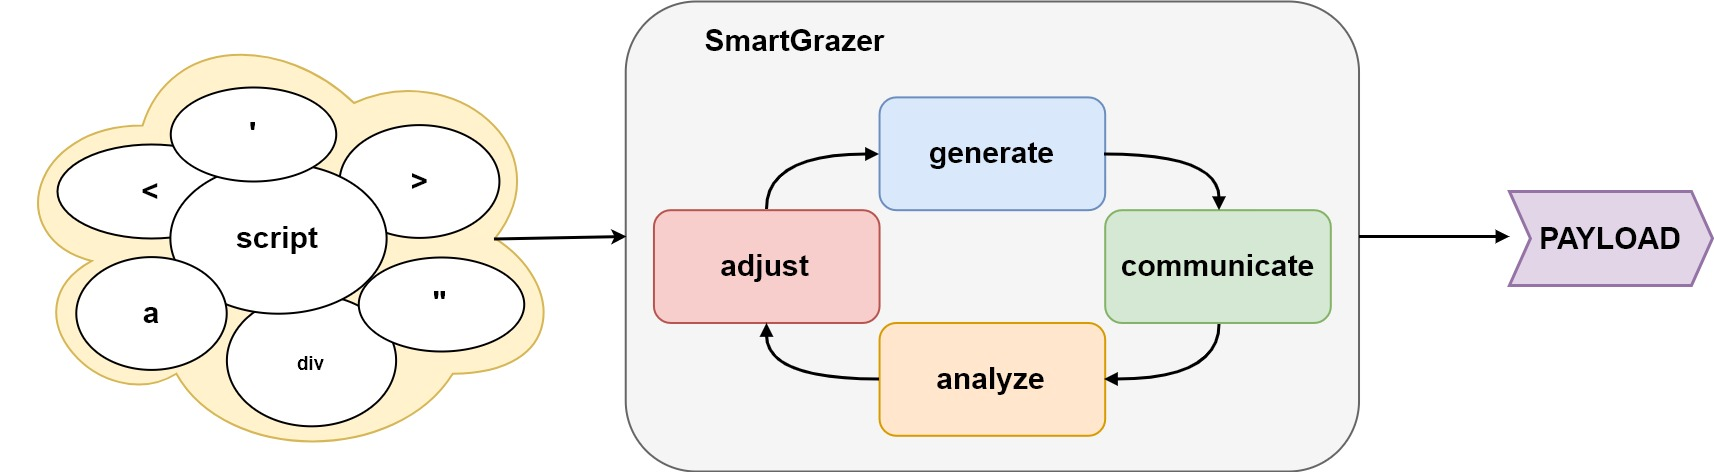
\includegraphics[width=\textwidth]{contents/images/SmartGrazerBirdView}
	\caption{Konzept: Grundsätzliche Vorgehensweise von SmartGrazer}
	\label{fig:SmartGrazerBirdView}
\end{figure}


\subsection{Definition: Payload-Elemente}
Ein Payload-Element kann entweder eine Zeichenkette (Text oder Schlüsselwort) oder ein Zeichen als Bestandteil von HTML oder JavaScript sein.

Während der Implementierung von SmartGrazer werden Elemente im Dezimalformat gespeichert und geladen. Dieser Wert ist eindeutig und wird während der Ausführung des Programms als Schlüssel (``key'') zur Identifizierung von Elementen verwendet. Dies hat den Vorteil, dass Steuerzeichen, wie beispielsweise das Tabulator-Zeichen  ``\lstinline[language=html]!\t!'', problemlos in Konfigurationsdateien gespeichert werden können. Das Zeichen (``value'') wird bei der Initialisierung des Elements aus dem Schlüssel errechnet.
Eine weitere Eigenschaft eines Payload-Elements bestimmt den Verwendungszweck (``usage''), dem das Element zugewiesen werden kann. Dementsprechend kann sowohl ein Leerzeichen als auch ein Tabulator-Zeichen als Weißraum in Payloads verwendet werden. Einigen Elementen können auch mehrere Verwendungen zugesprochen werden.
Beispielsweise wird das Plus-Zeichen ``+'' im Rahmen der URL-Kodierung als Leerzeichen  verwendet und gleichzeitig als Rechenoperand im JavaScript-Kontext.

%Ein Beispiel wäre das Plus-Zeichen, welche als ein Leerzeichen in der \ac{URL}-Kodierung oder für Rechenoperationen im JavaScript-Kontext verwendet werden können.

Um die Generatoren untereinander austauschen zu können, werden alle Payloads so generiert, dass diese in ihre vorhandenen Elemente aufgeteilt werden können.

\begin{figure}[htbp] 
	\centering
	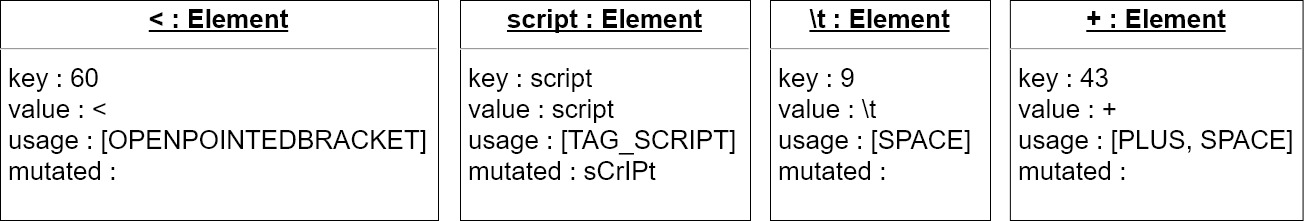
\includegraphics[width=\textwidth]{contents/images/SmartGrazerElementDefinition}
	\caption{Definition: Payload-Elemente als Objekte}
	\label{fig:element-definition}
\end{figure}

In den folgenden Kapiteln wird erläutert, wie die einzelnen Phasen (Generierung, Kommunikation, Analyse und Anpassung) realisiert worden sind. Im Anschluss daran werden in Kapitel \ref{sec:implementation_misc} weitere Details der fertigen Implementierung vorgestellt.